% Options for packages loaded elsewhere
\PassOptionsToPackage{unicode}{hyperref}
\PassOptionsToPackage{hyphens}{url}
%
\documentclass[
  american,
  man,floatsintext]{apa7}
\usepackage{lmodern}
\usepackage{amssymb,amsmath}
\usepackage{ifxetex,ifluatex}
\ifnum 0\ifxetex 1\fi\ifluatex 1\fi=0 % if pdftex
  \usepackage[T1]{fontenc}
  \usepackage[utf8]{inputenc}
  \usepackage{textcomp} % provide euro and other symbols
\else % if luatex or xetex
  \usepackage{unicode-math}
  \defaultfontfeatures{Scale=MatchLowercase}
  \defaultfontfeatures[\rmfamily]{Ligatures=TeX,Scale=1}
\fi
% Use upquote if available, for straight quotes in verbatim environments
\IfFileExists{upquote.sty}{\usepackage{upquote}}{}
\IfFileExists{microtype.sty}{% use microtype if available
  \usepackage[]{microtype}
  \UseMicrotypeSet[protrusion]{basicmath} % disable protrusion for tt fonts
}{}
\makeatletter
\@ifundefined{KOMAClassName}{% if non-KOMA class
  \IfFileExists{parskip.sty}{%
    \usepackage{parskip}
  }{% else
    \setlength{\parindent}{0pt}
    \setlength{\parskip}{6pt plus 2pt minus 1pt}}
}{% if KOMA class
  \KOMAoptions{parskip=half}}
\makeatother
\usepackage{xcolor}
\IfFileExists{xurl.sty}{\usepackage{xurl}}{} % add URL line breaks if available
\IfFileExists{bookmark.sty}{\usepackage{bookmark}}{\usepackage{hyperref}}
\hypersetup{
  pdftitle={Cognitive Load Reduces Reason-Giving in a Moral Dumbfounding Task},
  pdfauthor={Blinded1, Blinded2, Blinded1, \& Blinded1},
  pdflang={en-US},
  pdfkeywords={moral dumbfounding, morality, cognitive load, dual-processes},
  hidelinks,
  pdfcreator={LaTeX via pandoc}}
\urlstyle{same} % disable monospaced font for URLs
\usepackage{graphicx,grffile}
\makeatletter
\def\maxwidth{\ifdim\Gin@nat@width>\linewidth\linewidth\else\Gin@nat@width\fi}
\def\maxheight{\ifdim\Gin@nat@height>\textheight\textheight\else\Gin@nat@height\fi}
\makeatother
% Scale images if necessary, so that they will not overflow the page
% margins by default, and it is still possible to overwrite the defaults
% using explicit options in \includegraphics[width, height, ...]{}
\setkeys{Gin}{width=\maxwidth,height=\maxheight,keepaspectratio}
% Set default figure placement to htbp
\makeatletter
\def\fps@figure{htbp}
\makeatother
\setlength{\emergencystretch}{3em} % prevent overfull lines
\providecommand{\tightlist}{%
  \setlength{\itemsep}{0pt}\setlength{\parskip}{0pt}}
\setcounter{secnumdepth}{-\maxdimen} % remove section numbering
% Make \paragraph and \subparagraph free-standing
\ifx\paragraph\undefined\else
  \let\oldparagraph\paragraph
  \renewcommand{\paragraph}[1]{\oldparagraph{#1}\mbox{}}
\fi
\ifx\subparagraph\undefined\else
  \let\oldsubparagraph\subparagraph
  \renewcommand{\subparagraph}[1]{\oldsubparagraph{#1}\mbox{}}
\fi
% Manuscript styling
\usepackage{upgreek}
\captionsetup{font=singlespacing,justification=justified}

% Table formatting
\usepackage{longtable}
\usepackage{lscape}
% \usepackage[counterclockwise]{rotating}   % Landscape page setup for large tables
\usepackage{multirow}		% Table styling
\usepackage{tabularx}		% Control Column width
\usepackage[flushleft]{threeparttable}	% Allows for three part tables with a specified notes section
\usepackage{threeparttablex}            % Lets threeparttable work with longtable

% Create new environments so endfloat can handle them
% \newenvironment{ltable}
%   {\begin{landscape}\centering\begin{threeparttable}}
%   {\end{threeparttable}\end{landscape}}
\newenvironment{lltable}{\begin{landscape}\centering\begin{ThreePartTable}}{\end{ThreePartTable}\end{landscape}}

% Enables adjusting longtable caption width to table width
% Solution found at http://golatex.de/longtable-mit-caption-so-breit-wie-die-tabelle-t15767.html
\makeatletter
\newcommand\LastLTentrywidth{1em}
\newlength\longtablewidth
\setlength{\longtablewidth}{1in}
\newcommand{\getlongtablewidth}{\begingroup \ifcsname LT@\roman{LT@tables}\endcsname \global\longtablewidth=0pt \renewcommand{\LT@entry}[2]{\global\advance\longtablewidth by ##2\relax\gdef\LastLTentrywidth{##2}}\@nameuse{LT@\roman{LT@tables}} \fi \endgroup}

% \setlength{\parindent}{0.5in}
% \setlength{\parskip}{0pt plus 0pt minus 0pt}

% Overwrite redefinition of paragraph and subparagraph by the default LaTeX template
% See https://github.com/crsh/papaja/issues/292
\makeatletter
\renewcommand{\paragraph}{\@startsection{paragraph}{4}{\parindent}%
  {0\baselineskip \@plus 0.2ex \@minus 0.2ex}%
  {-1em}%
  {\normalfont\normalsize\bfseries\itshape\typesectitle}}

\renewcommand{\subparagraph}[1]{\@startsection{subparagraph}{5}{1em}%
  {0\baselineskip \@plus 0.2ex \@minus 0.2ex}%
  {-\z@\relax}%
  {\normalfont\normalsize\itshape\hspace{\parindent}{#1}\textit{\addperi}}{\relax}}
\makeatother

% \usepackage{etoolbox}
\makeatletter
\patchcmd{\HyOrg@maketitle}
  {\section{\normalfont\normalsize\abstractname}}
  {\section*{\normalfont\normalsize\abstractname}}
  {}{\typeout{Failed to patch abstract.}}
\patchcmd{\HyOrg@maketitle}
  {\section{\protect\normalfont{\@title}}}
  {\section*{\protect\normalfont{\@title}}}
  {}{\typeout{Failed to patch title.}}
\makeatother

\usepackage{xpatch}
\makeatletter
\xapptocmd\appendix
  {\xapptocmd\section
    {\addcontentsline{toc}{section}{\appendixname\ifoneappendix\else~\theappendix\fi\\: #1}}
    {}{\InnerPatchFailed}%
  }
{}{\PatchFailed}
\keywords{moral dumbfounding, morality, cognitive load, dual-processes\newline\indent Word count: 3,747}
\usepackage{csquotes}
\raggedbottom
\ifxetex
  % Load polyglossia as late as possible: uses bidi with RTL langages (e.g. Hebrew, Arabic)
  \usepackage{polyglossia}
  \setmainlanguage[variant=american]{english}
\else
  \usepackage[shorthands=off,main=american]{babel}
\fi

\title{Cognitive Load Reduces Reason-Giving in a Moral Dumbfounding Task}
\author{Blinded\textsuperscript{1}, Blinded\textsuperscript{2}, Blinded\textsuperscript{1}, \& Blinded\textsuperscript{1}}
\date{}


\shorttitle{Cognitive Load and Moral Dumbfounding}

\authornote{

Correspondence concerning this article should be addressed to Blinded, Blinded. E-mail: Blinded

}

\affiliation{\vspace{0.5cm}\textsuperscript{1} Blinded\\\textsuperscript{2} Blinded}

\abstract{%
Moral dumbfounding occurs when people defend a moral judgment, without reasons in support of this judgment. The phenomenon has been influential in moral psychology, however, despite its influence, it remains poorly understood. Based on the notion that cognitive load enhances biases and shortcomings in human judgment when elaboration is beneficial, we hypothesized that under cognitive load, people would be less likely to provide reasons for a judgment and more likely to be dumbfounded. In a pre-registered study (N = 1686) we tested this prediction. Our findings suggest that cognitive load reduces reason-giving, leading to increases in dumbfounding. Our results provide new insights into the phenomenon of moral dumbfounding while also advancing theory in moral psychology.
}



\begin{document}
\maketitle

Moral dumbfounding occurs when people defend a moral judgment even though they cannot provide a reason in support of this judgment (Haidt et al., 2000; Haidt, 2001; see also McHugh, et al., 2017, 2020). It has traditionally been seen as evidence for intuitionist and dual-process theories of moral judgment (e.g., Crockett, 2013; Cushman, 2013; Cushman, Young, \& Greene, 2010; Greene, 2008; Haidt, 2001; Prinz, 2005; though this narrative has been contested, e.g., Guglielmo, 2018; Royzman et al., 2015). Despite the influence of moral dumbfounding on the morality literature, the phenomenon is not well understood. Here we present a pre-registered test of one prediction of a dual-process explanation of moral dumbfounding.

\hypertarget{moral-dumbfounding-a-dual-process-perspective}{%
\section{Moral Dumbfounding: A Dual-Process Perspective}\label{moral-dumbfounding-a-dual-process-perspective}}

Drawing on dual-process theories of reasoning and moral judgment (e.g., Greene, 2008; Bago \& De Neys, 2019; Brand, 2016; Cushman, 2013), we propose that moral dumbfounding occurs as a result of a conflict in dual-processes (Bonner \& Newell, 2010; De Neys, 2012; De Neys \& Glumicic, 2008; Evans, 2007; see also De Neys \& Pennycook, 2019). In classic dual-process reasoning accounts, conflicts occur when a habitual/intuitive response is different from a response that results from deliberation (Bonner \& Newell, 2010). Examples of such conflicts include base rate neglect problems (Bonner \& Newell, 2010; De Neys, 2012; De Neys \& Glumicic, 2008; Evans, 2007), the conjunction fallacy (De Neys, 2012; Tversky \& Kahneman, 1983), and perhaps most relevant to the current discussion, a seemingly irrational but persistent unwillingness to contact various symbolically \enquote{contaminated} objects, despite assurances these items are sanitary (e.g., items believed to have had prior contact with: an AIDS victim, someone who had been in a car accident, or a murderer, see Rozin et al., 1994; Lerner \& Goldberg, 1999). We note that the original, unpublished dumbfounding manuscript included tasks closely resembling this final example (Haidt et al., 2000).

In line with the above, we propose that dumbfounding occurs when a habitual (moral judgment) response is in conflict with a deliberative response. In studies of moral dumbfounding, following an initial judgment, there are typically three responses available to participants: (1) providing a reason or justification for a judgment (henceforth reason-giving); (2) accepting counter-arguments and rating particular behaviors as \enquote{not wrong} (nothing-wrong); (3) maintaining a judgment without justification or reasons (dumbfounding). Both reason-giving and nothing-wrong can be accounted for by existing approaches to moral judgment (e.g., Cushman, 2013), and while reason-giving is the most common response, dumbfounding is reliably observed (see McHugh et al., 2017, 2020) and remains an anomaly.

Drawing on existing theorizing (Cushman, 2013; Haidt, 2001; McHugh et al., 2022), we assume that making a moral judgment is an intuitive/habitual response involving relatively little deliberation, while reason-giving requires greater deliberation (a deliberative response). In this view, conflict occurs when deliberation fails to identify reasons for a judgment, and its resolution depends on the availability of cognitive resources for deliberation -- further deliberation may identify relevant reasons. Alternatively, participants may resolve the conflict by accepting the arguments presented and changing their judgment (nothing-wrong). We propose that dumbfounding is observed when this conflict cannot be resolved. We hypothesize that nothing-wrong involves more deliberation than dumbfounding but less deliberation than reason-giving. The hypothesized relative amounts of deliberation for each response are outlined in Figure 1. We note that this explanation is not unique to dual-process approaches, but is also consistent with a unimodal (Kruglanski \& Gigerenzer, 2011) or categorization (McHugh et al., 2022) approaches, both of which predict that lower processing capacity reduces reason-giving, and increases dumbfounding.

\begin{figure}
\centering
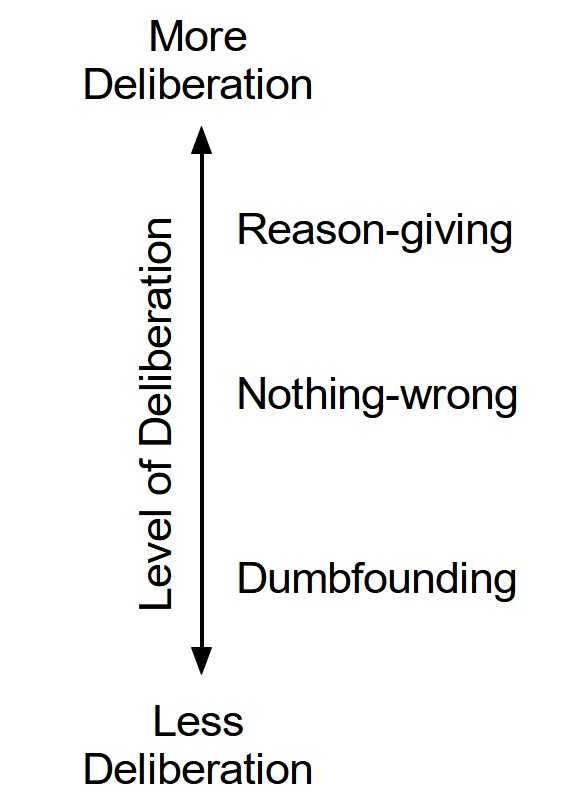
\includegraphics[width=2.60417in,height=\textheight]{../resources/images/responses_figure4.jpg}
\caption{Hypothesized relationship between deliberation and responses in the dumbfounding paradigm}
\end{figure}

This account of moral dumbfounding affords a clear testable hypothesis: under manipulations that affect the availability of resources for deliberation, responses in the moral dumbfounding paradigm should evidence variation in frequency of deliberative versus habitual responses. Cognitive load manipulations -- such as completing an attention/memory task simultaneously with a primary task -- have been shown to inhibit deliberative responding (De Neys \& Glumicic, 2008; Evans \& Curtis-Holmes, 2005; Evans \& Stanovich, 2013; Schmidt, 2016). We have identified reason-giving as involving more deliberation than alternative responses in the dumbfounding paradigm. Thus, we predict that a cognitive load manipulation should inhibit reason-giving in a moral dumbfounding task, leading to an increase in habitual responding, such as dumbfounding or nothing-wrong.

\hypertarget{the-current-research}{%
\section{The Current Research}\label{the-current-research}}

Our primary prediction is that a cognitive load manipulation will inhibit people's ability to provide reasons for their judgment, leading to greater habitual responses (either dumbfounding or nothing wrong or both). We present a pre-registered study to test this prediction of a conflict in dual-process explanation of moral dumbfounding. We experimentally manipulated cognitive load, and predicted that this cognitive load manipulation will inhibit people's ability to provide reasons for their judgment, leading to greater habitual responses (either nothing wrong or dumbfounding or both).

Our cognitive load manipulation involved a secondary task requiring participants to pay attention to a stream of numbers on the screen while completing the moral judgment task. We conducted a series of pilot studies (see Supplement Studies S1 - S5) involving two different memory tasks. The effectiveness of these memory tasks in manipulating cognitive load was unclear, and it is possible that participants could cheat on these memory tasks (particularly for online samples). As such, we selected a cognitive load manipulation that required participants to pay attention to a secondary task (rather than a memory task) while engaged in the primary judgment task (in line with Greene et al., 2008).

The data for this study (and all pilot studies), as well as the analysis code for all studies, and full materials for this study including jsPsych script are publicly available at \color{blue}\url{https://osf.io/fcd5r/?view_only=9fb6e506e53340c189b98453bb2b6eaf}\color{black}. This study was pre-registered and the pre-registration is available at \color{blue}\url{https://aspredicted.org/XZP_UHW}\color{black}. All analyses were conducted in R (R Core Team, 2021), see analysis code for full list of packages.

\hypertarget{method}{%
\subsection{Method}\label{method}}

\hypertarget{participants-and-design}{%
\subsubsection{Participants and design}\label{participants-and-design}}

This study was a between subjects design. The dependent variable was rates of reason-giving/dumbfounding (measured using the critical slide with 3 response options: 1: reason-giving; 2: nothing-wrong; 3: dumbfounded response - admission). The primary independent variable was cognitive load with two levels: present and absent. To manipulate cognitive load, a stream of numbers scrolled across the screen above the question text, and participants were required to pay attention to how many times they saw a given number. The scenario served as a secondary independent variable, we used four scenarios: \emph{Julie and Mark (Incest)}, \emph{Jennifer (Cannibal)}, \emph{Trolley}, \emph{Heinz} (see Supplementary Materials for full text of each).

A total sample of 1899 participants (984 female, 876 male, 17 non-binary, 1 other, 5 prefer not to say; \emph{M}\textsubscript{age} = 43.22, min = 18, max = 84, \emph{SD} = 15.85) started the survey. Participants in this sample were recruited from Prolific (\emph{n\textsubscript{UK}} = 963, \emph{n\textsubscript{US}} = 936).\footnote{A priori power analysis indicated that, for the primary research question (the influence of cognitive load on dumbfounded responding), in order to detect a large effect size (\emph{V} = .35) with 80\% power, a sample of \emph{N} = 79 participants was required; in order to detect a medium effect size (\emph{V} = .21) with 80\% power a sample of \emph{N} = 218 participants was required; in order to detect a small effect size (\emph{V} = .07) with 80\% power a sample of \emph{N} = 1966 was required.}

Participants who failed both manipulation checks (\emph{n} = 7) or who had missing data for the measures of interest were removed, leaving a total sample of 1686 participants (867 female, 799 male, 14 non-binary, 1 other, 5 prefer not to say; \emph{M}\textsubscript{age} = 43.81, min = 18, max = 83, \emph{SD} = 15.76), \emph{n\textsubscript{UK}} = 842, \emph{n\textsubscript{US}} = 844.

\hypertarget{procedure-and-materials}{%
\subsubsection{Procedure and materials}\label{procedure-and-materials}}

Data were collected using an online questionnaire developed with \emph{jsPsych} and distributed with \emph{cognition.run}. Participants were presented with one of four moral scenarios (\emph{Julie and Mark}, \emph{Jennifer}, \emph{Trolley}, \emph{Heinz}, see supplementary materials for full wording), previously used in studies of moral dumbfounding (McHugh et al., 2017). Participants rated on a 7-point Likert scale how right or wrong the behavior of the character in the scenario was (where, 1 = \emph{Morally wrong}; 4 = \emph{neutral}; 7 = \emph{Morally right}), and were given an opportunity to provide reasons for their judgment. Following this, participants were presented with a series of counter-arguments, which refute commonly used justifications for rating the behavior as \enquote{wrong} (see supplementary materials for full text of scenarios and all counter-arguments).

Dumbfounding was measured using the critical slide (developed by McHugh et al., 2017). This contained a statement defending the behavior and a question as to how the behavior could be wrong (e.g., \enquote{Julie and Mark's behavior did not harm anyone, how can there be anything wrong with what they did?}). There were three possible answer options: (a) \enquote{It's wrong, and I can provide a valid reason} (reasons); (b) \enquote{It's wrong, but I can't think of a reason} (an admission of not having reasons); (c) \enquote{There is nothing wrong}. The order of these response options was randomized. Participants who selected (a) were prompted to type a reason. The selecting of an option (b), the admission of not having reasons, was taken to be a dumbfounded response.\footnote{This measure avoids the potential confounding influence of qualitative differences between different response types; that is, participants indicate whether they can provide reasons for their judgments or not, and this is our measure (not whether or not they actually provide reasons, as this different type of response would not be comparable to a dumbfounded response).}
We note that this measure provides a conservative measure of dumbfounded responding {[}see McHugh et al. (2017) for discussion). A key advantage of this measure of dumbfounding is its suitability for use with cognitive load manipulations. The task requirements for each of the three response options are qualitatively the same (selecting a response), eliminating the potential confounding influence of different types of task requirements. Importantly, participants who selected (a) were only prompted to provide a reason after their response to the critical slide had been submitted and recorded, and the survey had proceeded to the next page. Participants did not know they would be required to provide a reason prior to the presentation of this prompt.

We included a video stream of numbers scrolling above the question text for our cognitive load manipulation, drawing on Greene et al. (2008). The video was wide enough to display 3 numbers at a time, and the numbers scrolled past at a speed of 2 numbers per second. Participants were asked to attend to and report (on a subsequent page) how many times a particular number appeared in the stream, while answering the target question. Following an initial training task, the video was presented while participants made their initial judgments, while they responded to the critical slide, and while they were providing their revised judgments.

Two attention check tasks were included for all participants, these included a brief paragraph of text where instructions for the correct response were embedded within the text. The wording of the text was misleading such that if participants skimmed or only read some of the text they would likely provide an incorrect response.

Participants clicked on the survey link and were randomly assigned to either the experimental condition or the control condition, within which they were randomly presented with one of the four scenarios. The study was complete within 5 minutes.

\hypertarget{results}{%
\subsection{Results}\label{results}}

One thousand three hundred sixty-five participants (80.96\%) rated the behavior described as wrong initially, and one thousand three hundred forty three participants (79.66\%) rated the behavior as wrong at the end of the task. Initial ratings (\emph{M} = 2.26, \emph{SD} = 1.63) were significantly more severe than revised ratings (\emph{M} = 2.34, \emph{SD} = 1.66), \emph{t}(1685) = -2.69, \emph{p} = .007; \emph{d} = 0.07. Inspection of the binned judgments revealed that two hundred (11.86\%) participants changed the valence of their judgments, breakdown of the changes in judgments is in Table 16 (full sample) and Table 17 (by scenario) in the supplementary materials.

A 2 \(\times\) 2 factorial ANOVA revealed significant differences in initial judgments depending on both condition \emph{F}(1, 1678) = 26.65, \emph{p} \textless{} .001, partial \(\eta\)\textsuperscript{2} = .016, and scenario \emph{F}(3, 1678) = 69.30, \emph{p} \textless{} .001, partial \(\eta\)\textsuperscript{2} = .110. Participants under cognitive load were significantly (\emph{p} \textless{} .001) less harsh in their judgments (\emph{M} = 2.46, \emph{SD} = 1.75) than those in the control condition (\emph{M} = 2.07, \emph{SD} = 1.49). Participants rated \emph{Jennifer} as the most wrong (\emph{M} = 1.53, \emph{SD} = 1.13), followed by \emph{Julie and Mark} (\emph{M} = 2.05, \emph{SD} = 1.65, \emph{p} \textless{} .001), then \emph{Heinz} (\emph{M} = 2.49, \emph{SD} = 1.65, \emph{p} \textless{} .001), with \emph{Trolley} receiving the least severe judgment (\emph{M} = 2.98, \emph{SD} = 1.69, \emph{p} \textless{} .001). There was no significant condition \(\times\) scenario interaction \emph{F}(3, 1678) = 0.46, \emph{p} = .708, partial \(\eta\)\textsuperscript{2} \textless{} .001.

A 2 \(\times\) 2 factorial ANOVA revealed significant differences in revised judgments depending on both condition \emph{F}(1, 1678) = 12.82, \emph{p} \textless{} .001, partial \(\eta\)\textsuperscript{2} = .008, and scenario \emph{F}(3, 1678) = 80.69, \emph{p} \textless{} .001, partial \(\eta\)\textsuperscript{2} = .126. Participants under cognitive load were significantly (\emph{p} \textless{} .001) less harsh in their judgments (\emph{M} = 2.47, \emph{SD} = 1.71) than those in the control condition (\emph{M} = 2.20, \emph{SD} = 1.59). Participants rated \emph{Jennifer} as the most wrong (\emph{M} = 1.54, \emph{SD} = 1.12), followed by \emph{Julie and Mark} (\emph{M} = 2.15, \emph{SD} = 1.73, \emph{p} \textless{} .001), then \emph{Heinz} (\emph{M} = 2.52, \emph{SD} = 1.58, \emph{p} = .003), with \emph{Trolley} receiving the least severe judgment (\emph{M} = 3.14, \emph{SD} = 1.72, \emph{p} \textless{} .001). There was no significant condition \(\times\) scenario interaction \emph{F}(3, 1678) = 1.34, \emph{p} = .260, partial \(\eta\)\textsuperscript{2} = .002.

Dumbfounding was recorded using the critical slides, participants who selected the admission of not having reasons on the critical slide were identified as dumbfounded. Four hundred and seventeen participants (24.73\%) selected \enquote{It's wrong but I can't think of a reason}. One thousand and thirty-two participants (61.21\%) selected \enquote{It's wrong and I can provide a valid reason}; and two hundred and thirty-seven participants (14.06\%) selected \enquote{There is nothing wrong}.

A chi-squared test for independence revealed a significant association between experimental condition and response to the critical slide, \(\chi\)\textsuperscript{2}(2, \emph{N} = 1686) = 25.48, \emph{p} \textless{} .001, \emph{V} = 0.12, the observed power was 0.997. As predicted, under cognitive load fewer participants (458; 55.45\%) provided reasons than in the control condition (574; 66.74\%), and more participants (245; 29.66\%) selected \enquote{It's wrong but I can't think of a reason.} than in the control group (172; 20\%). The responses to the critical slide for the experimental group (\emph{N} = 826) and the control group (\emph{N} = 860) are displayed in Figure~\ref{fig:S6ch5S6fig1criticalconditionb}. The observed counts, expected counts and standardised residuals are displayed in Table~\ref{tab:S6tab1dumb}.

\newpage

\begin{figure}
\centering
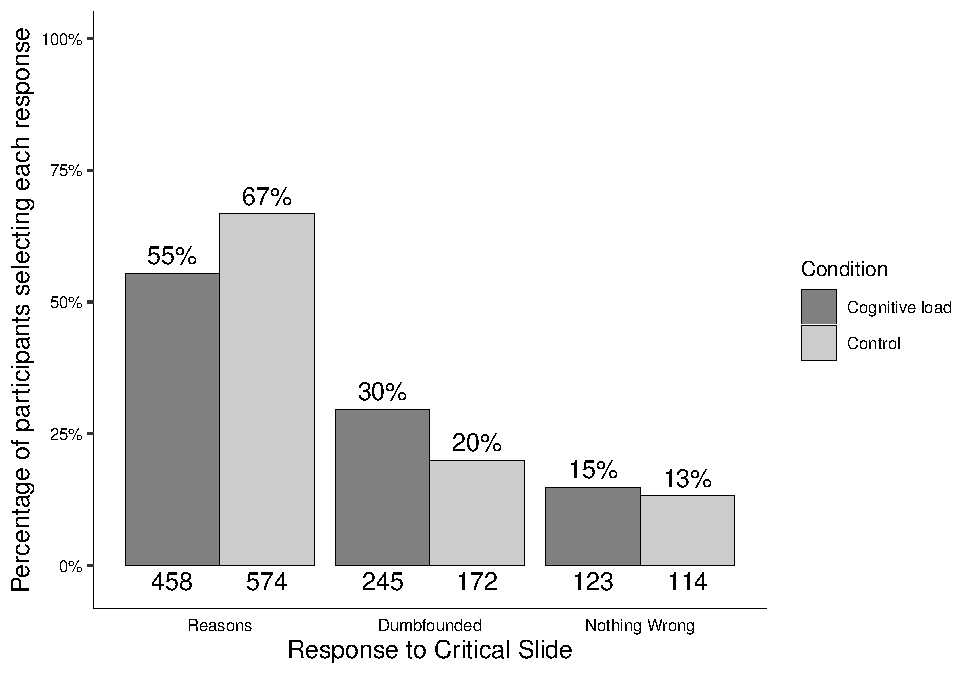
\includegraphics{cog_load_in_chunks_files/figure-latex/S6ch5S6fig1criticalconditionb-1.pdf}
\caption{\label{fig:S6ch5S6fig1criticalconditionb}Responses to critical slide depending on cognitive load}
\end{figure}

\begin{table}[tbp]

\begin{center}
\begin{threeparttable}

\caption{\label{tab:S6tab1dumb}Observed counts, expected counts, and standardised residuals for each response to the critical slide depending on cognitive load (full sample)}

\begin{tabular}{llcc}
\toprule
 & \multicolumn{1}{c}{} & \multicolumn{1}{c}{Cognitive Load} & \multicolumn{1}{c}{Control}\\
\midrule
Observed count & Reasons & 458 & 574\\
 & Dumbfounded & 245 & 172\\
 & Nothing Wrong & 123 & 114\\
Expected count & Reasons & 505.59 & 526.41\\
 & Dumbfounded & 204.3 & 212.7\\
 & Nothing Wrong & 116.11 & 120.89\\
Standardised residuals & Reasons & -4.76** & 4.76**\\
 & Dumbfounded & 4.6** & -4.6**\\
 & Nothing Wrong & 0.97 & -0.97\\
\bottomrule
\addlinespace
\end{tabular}

\begin{tablenotes}[para]
\normalsize{\textit{Note.} * = sig. at \emph{p} < .05; ** = sig. at \emph{p} < .001}
\end{tablenotes}

\end{threeparttable}
\end{center}

\end{table}

\newpage

This pattern was observed for all scenarios individually with the exception of \emph{Julie and Mark}, which showed no association between experimental condition and cognitive load, \(\chi\)\textsuperscript{2}(2, \emph{N} = 418) = 0.49, \emph{p} = .783, \emph{V} = 0.25, power = 0.601. The association was significant for \emph{Jennifer} \(\chi\)\textsuperscript{2}(2, \emph{N} = 418) = 17.33, \emph{p} \textless{} .001, \emph{V} = 0.24, power = 0.623, \emph{Trolley} \(\chi\)\textsuperscript{2}(2, \emph{N} = 418) = 10.95, \emph{p} = .004, \emph{V} = 0.25, power = 0.614, and Heinz, \(\chi\)\textsuperscript{2}(2, \emph{N} = 418) = 7.16, \emph{p} = .028, \emph{V} = 0.25, power = 0.608, see Figure~\ref{fig:S6ch5S6fig2criticalconditionb}. Supplementary Tables 20-23 show the direction of the effect for each scenario. Under cognitive load, fewer participants provided reasons and more participants provided a dumbfounded response for \emph{Jennifer}, \emph{Trolley}, and \emph{Heinz}

\begin{figure}
\centering
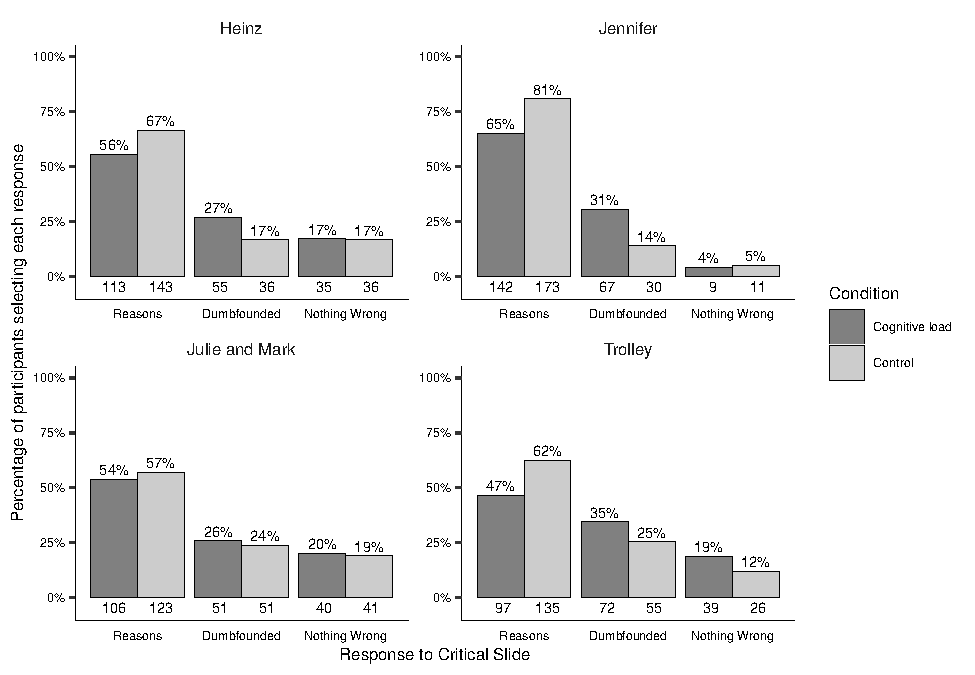
\includegraphics{cog_load_in_chunks_files/figure-latex/S6ch5S6fig2criticalconditionb-1.pdf}
\caption{\label{fig:S6ch5S6fig2criticalconditionb}Responses to critical slide and for the experimental group and the control group for each scenario}
\end{figure}

A chi-squared test for independence revealed a significant association between scenario and response to the critical slide, \(\chi\)\textsuperscript{2}(6, \emph{N} = 1686) = 61.34, \emph{p} \textless{} .001, \emph{V} = 0.19, the observed power was 1. Participants were significantly more likely to select \enquote{There is nothing wrong} for \emph{Julie and Mark} (\emph{p} = .002), more likely to provide reasons (\emph{p} = .002) and less likely to select \enquote{There is nothing wrong} (\emph{p} \textless{} .001) for Jennifer, and more likely to be dumbfounded by \emph{Trolley} (\emph{p} = .031).

A multinomial logistic regression was conducted to test the effects of cognitive load and scenario on dumbfounded responding. Overall the model was significant, \(\chi\)\textsuperscript{2}(8, \emph{N} = 1686) = 95.9, \emph{p} \textless{} .001, and explained between 6.07\% (Cox and Snell R square) and 7.22\% (Nadelkerke R squared) of the variance in responses to the critical slide, the observed power was 1. Participants in the control condition were significantly less likely to provide a dumbfounded response than to provide reasons, Wald = 25.04, \emph{p} \textless{} .001, \emph{OR} = 0.55, 95\% CI {[}0.44, 0.70{]}, in addition, participants in the control condition were also signifcantly less likely to select \enquote{There is nothing wrong}, than to provide reasons, Wald = 5.23, \emph{p} = .022, \emph{OR} = 0.71, 95\% CI {[}0.54, 0.95{]}. For \emph{Jennifer}, participants were significantly less likely to select \enquote{There is nothing wrong} than to provide a reason, Wald = 30.87, \emph{p} \textless{} .001, \emph{OR} = 0.23, 95\% CI {[}0.13, 0.38{]}; while for \emph{Trolley} participants were significantly more likely to present as dumbfounded than to provide a reason, Wald = 6.89, \emph{p} = .009, \emph{OR} = 1.55, 95\% CI {[}1.12, 2.14{]}.

\newpage

\hypertarget{discussion}{%
\section{Discussion}\label{discussion}}

The present research aimed to add to the literature on moral judgments by offering new insights into factors that prompt moral dumbfounding. We hypothesized that under cognitive load, participants would be less likely to provide reasons and more likely to present as dumbfounded (or to select nothing-wrong). When participants engaged in a secondary task while completing a dumbfounding task reason-giving was inhibited for three out of four scenarios tested. Overall we find evidence that in situations where the resources available for deliberation are limited (as when cognitive load is high), reason-giving is reduced, and moral dumbfounding is more likely. This key finding is consistent with previous work demonstrating that cognitive load inhibits deliberative responding (De Neys, 2006; Evans \& Curtis-Holmes, 2005).

\hypertarget{implications-limitations-and-future-directions}{%
\subsection{Implications, Limitations, and Future Directions}\label{implications-limitations-and-future-directions}}

These studies offer new understandings of the phenomenon of moral dumbfounding. While our studies illustrate the complexity of attempting to understand moral judgments, we do demonstrate some reliable patterns that offer support to our core theoretically-informed hypotheses. Furthermore, these studies showcase a methodology for measuring dumbfounding under different empirical conditions, offering a path for future researchers to explore the role of other contextual and individual difference variables in influencing moral dumbfounding.

From a theoretical perspective our findings are consistent with a dual-process explanation of moral dumbfounding, whereby dumbfounding occurs when an intuitive/habitual response is in conflict with a deliberative response (Evans, 2007; again we note that the assumption of dual-processes is not necessarily required, and that this prediction is also consistent with the unimodel, Kruglanski \& Gigerenzer, 2011; or categorization approaches McHugh et al., 2022). In line with existing theorizing on moral judgments (Cushman, 2013; McHugh et al., 2022; Railton, 2017), we propose that an individual may make an intuitive judgment and that subsequent attempts to identify reasons for this judgment occur through deliberation. If deliberation is unsuccessful and the individual does not revise their judgment, dumbfounding is observed. In support of this explanation, our studies demonstrated that by reducing the cognitive resources available for deliberation, reason-giving was reduced and dumbfounding increased.

These findings have relevance for society more broadly. Moral considerations inform a range of behaviors and decisions, both at the individual level and at the societal level (Sinnott-Armstrong, Young, \& Cushman, 2010). It is likely that moral dumbfounding may be a contributing factor to moral disagreement on contentious issues. Our studies provide evidence that dumbfounding may be more prevalent in situations that constrain people's ability to engage in deliberation. In practice, this suggests that when discussing contentious moral issues, disagreement through dumbfounding may be reduced by ensuring conditions suitable for deliberation (e.g., avoiding emotionally charged, high-pressure environments).

Our results do display some unexplained variability with the \emph{classic} dumbfounding scenario (\emph{Julie and Mark}) showing no change in responding with increased cognitive load (we note that the pilot studies used only this scenario and also showed mixed results). It may be possible to attribute some of this variability to methodological limitations. Classic studies of dual-process conflict are characterized by binary response options (an intuitive response contrasted with a deliberative response; Evans, 2007), whereas our studies included three response options that varied in their relative amount of deliberation. It is also possible that this variability reflects a lack of statistical power do detect small effects for the specific scenario.

However, is also possible that these results provide evidence that the conflict in dual-process explanation tested here is only part of the story, illustrating that moral dumbfounding displays high variability and context dependency (as with moral judgment more generally, see McHugh et al., 2022). A further complication is that responses in the dumbfounding paradigm may involve competing intuitions. For example, participants may have intuitions relating to the nature of moral knowledge, such as moral judgments should be justifiable by reasons, that may become salient during the course of the study. This means that, in addition to experiencing a conflict between habitual and deliberative responding, participants may also experience competing intuitions. Future research should unpack the influences of these competing intuitions.

While the studies presented here were in line with our theoretical predictions, we note that our samples were either student or online participants from Westernized countries, limiting the generalizability of our findings. While emerging research suggests that dumbfounding is observed in certain non-WEIRD populations (McHugh, Zhang, Karnatak, Lamba, \& Khokhlova, 2021), future research should test if the explanation tested here generalizes beyond Western contexts.

\hypertarget{conclusion}{%
\section{Conclusion}\label{conclusion}}

Moral dumbfounding occurs when people stubbornly maintain a moral judgment, even without reasons to support their judgments. To date, there are few studies that consider the causes of moral dumbfounding. Here, we test the idea that moral dumbfounding is more likely to occur when an individual is experiencing greater demands on their cognitive system, leaving less cognitive resources available for reasoning in complex moral dilemmas. The findings from the present research show that moral dumbfounding is more likely to occur under cognitive load, at least in some contexts. While these findings add new knowledge to the literature on moral dumbfounding, they also highlight the complexities of moral judgments. Further research is needed to better understand the factors that lead to dumbfounding, and, ultimately, how it might be reduced.
\newpage


\hypertarget{references}{%
\section{References}\label{references}}

\setlength{\parindent}{-0.5in}
\setlength{\leftskip}{0.5in}
\setlength{\parskip}{8pt}

\hypertarget{refs}{}
\leavevmode\hypertarget{ref-bago_intuitive_2019}{}%
Bago, B., \& De Neys, W. (2019). The intuitive greater good: Testing the corrective dual process model of moral cognition. \emph{Journal of Experimental Psychology: General}, \emph{148}(10), 1782--1801. \url{https://doi.org/10.1037/xge0000533}

\leavevmode\hypertarget{ref-bonner_conflict_2010}{}%
Bonner, C., \& Newell, B. R. (2010). In conflict with ourselves? An investigation of heuristic and analytic processes in decision making. \emph{Memory \& Cognition}, \emph{38}(2), 186--196. \url{https://doi.org/10.3758/MC.38.2.186}

\leavevmode\hypertarget{ref-brand_dualprocess_2016}{}%
Brand, C. (2016). \emph{Dual-Process Theories in Moral Psychology: Interdisciplinary Approaches to Theoretical, Empirical and Practical Considerations}. Springer.

\leavevmode\hypertarget{ref-crockett_models_2013}{}%
Crockett, M. J. (2013). Models of morality. \emph{Trends in Cognitive Sciences}, \emph{17}(8), 363--366. \url{https://doi.org/10.1016/j.tics.2013.06.005}

\leavevmode\hypertarget{ref-cushman_action_2013}{}%
Cushman, F. A. (2013). Action, Outcome, and Value A Dual-System Framework for Morality. \emph{Personality and Social Psychology Review}, \emph{17}(3), 273--292. \url{https://doi.org/10.1177/1088868313495594}

\leavevmode\hypertarget{ref-cushman_multisystem_2010}{}%
Cushman, F. A., Young, L., \& Greene, J. D. (2010). Multi-system Moral Psychology. In J. M. Doris (Ed.), \emph{The Moral Psychology Handbook} (pp. 47--71). Oxford; New York: Oxford University Press.

\leavevmode\hypertarget{ref-deneys_dual_2006}{}%
De Neys, W. (2006). Dual Processing in Reasoning: Two Systems but One Reasoner. \emph{Psychological Science}, \emph{17}(5), 428--433. \url{https://doi.org/10.1111/j.1467-9280.2006.01723.x}

\leavevmode\hypertarget{ref-deneys_bias_2012}{}%
De Neys, W. (2012). Bias and Conflict: A Case for Logical Intuitions. \emph{Perspectives on Psychological Science}, \emph{7}(1), 28--38. \url{https://doi.org/10.1177/1745691611429354}

\leavevmode\hypertarget{ref-deneys_conflict_2008}{}%
De Neys, W., \& Glumicic, T. (2008). Conflict monitoring in dual process theories of thinking. \emph{Cognition}, \emph{106}(3), 1248--1299. \url{https://doi.org/10.1016/j.cognition.2007.06.002}

\leavevmode\hypertarget{ref-deneys_logic_2019}{}%
De Neys, W., \& Pennycook, G. (2019). Logic, Fast and Slow: Advances in Dual-Process Theorizing. \emph{Current Directions in Psychological Science}, \emph{28}(5), 503--509. \url{https://doi.org/10.1177/0963721419855658}

\leavevmode\hypertarget{ref-evans_resolution_2007}{}%
Evans, J. S. B. T. (2007). On the resolution of conflict in dual process theories of reasoning. \emph{Thinking \& Reasoning}, \emph{13}(4), 321--339. \url{https://doi.org/10.1080/13546780601008825}

\leavevmode\hypertarget{ref-evans_rapid_2005}{}%
Evans, J. S. B. T., \& Curtis-Holmes, J. (2005). Rapid responding increases belief bias: Evidence for the dual-process theory of reasoning. \emph{Thinking \& Reasoning}, \emph{11}(4), 382--389. \url{https://doi.org/10.1080/13546780542000005}

\leavevmode\hypertarget{ref-evans_dualprocess_2013}{}%
Evans, J. S. B. T., \& Stanovich, K. E. (2013). Dual-Process Theories of Higher Cognition: Advancing the Debate. \emph{Perspectives on Psychological Science}, \emph{8}(3), 223--241. \url{https://doi.org/10.1177/1745691612460685}

\leavevmode\hypertarget{ref-greene_secret_2008}{}%
Greene, J. D. (2008). The Secret Joke of Kant's Soul. In \emph{Moral Psychology Volume 3: The neurosciences of morality: Emotion, brain disorders, and development} (pp. 35--79). Cambridge (Mass.): the MIT press.

\leavevmode\hypertarget{ref-greene_cognitive_2008}{}%
Greene, J. D., Morelli, S. A., Lowenberg, K., Nystrom, L. E., \& Cohen, J. D. (2008). Cognitive load selectively interferes with utilitarian moral judgment. \emph{Cognition}, \emph{107}(3), 1144--1154. \url{https://doi.org/10.1016/j.cognition.2007.11.004}

\leavevmode\hypertarget{ref-guglielmo_unfounded_2018}{}%
Guglielmo, S. (2018). Unfounded dumbfounding: How harm and purity undermine evidence for moral dumbfounding. \emph{Cognition}, \emph{170}, 334--337. \url{https://doi.org/10.1016/j.cognition.2017.08.002}

\leavevmode\hypertarget{ref-haidt_emotional_2001}{}%
Haidt, J. (2001). The emotional dog and its rational tail: A social intuitionist approach to moral judgment. \emph{Psychological Review}, \emph{108}(4), 814--834. \url{https://doi.org/10.1037/0033-295X.108.4.814}

\leavevmode\hypertarget{ref-haidt_moral_2000}{}%
Haidt, J., Björklund, F., \& Murphy, S. (2000). Moral dumbfounding: When intuition finds no reason. \emph{Unpublished Manuscript, University of Virginia}.

\leavevmode\hypertarget{ref-kruglanski_intuitive_2011}{}%
Kruglanski, A. W., \& Gigerenzer, G. (2011). Intuitive and deliberate judgments are based on common principles. \emph{Psychological Review}, \emph{118}(1), 97--109. \url{https://doi.org/10.1037/a0020762}

\leavevmode\hypertarget{ref-lerner_when_1999}{}%
Lerner, M. J., \& Goldberg, J. H. (1999). When Do Decent People Blame Victims? The Differing Effects of the Explicit/Rational and Implicit/Experiential Cognitive Systems. In S. Chaiken \& Y. Trope (Eds.), \emph{Dual-process Theories in Social Psychology} (pp. 627--640). Guilford Press.

\leavevmode\hypertarget{ref-mchugh_searching_2017a}{}%
McHugh, C., McGann, M., Igou, E. R., \& Kinsella, E. L. (2017). Searching for Moral Dumbfounding: Identifying Measurable Indicators of Moral Dumbfounding. \emph{Collabra: Psychology}, \emph{3}(1), 1--24. \url{https://doi.org/10.1525/collabra.79}

\leavevmode\hypertarget{ref-mchugh_reasons_2020}{}%
McHugh, C., McGann, M., Igou, E. R., \& Kinsella, E. L. (2020). Reasons or rationalizations: The role of principles in the moral dumbfounding paradigm. \emph{Journal of Behavioral Decision Making}, \emph{33}(3), 376--392. \url{https://doi.org/10.1002/bdm.2167}

\leavevmode\hypertarget{ref-mchugh_moral_2022}{}%
McHugh, C., McGann, M., Igou, E. R., \& Kinsella, E. L. (2022). Moral Judgment as Categorization (MJAC). \emph{Perspectives on Psychological Science}, \emph{17}(1), 131--152. \url{https://doi.org/10.1177/1745691621990636}

\leavevmode\hypertarget{ref-mchugh_just_2021}{}%
McHugh, C., Zhang, R., Karnatak, T., Lamba, N., \& Khokhlova, O. (2021). \emph{Just Wrong? Or just WEIRD? Investigating the prevalence of Moral Dumbfounding in non-Western samples}. PsyArXiv. \url{https://doi.org/10.31234/osf.io/zxfbj}

\leavevmode\hypertarget{ref-prinz_passionate_2005}{}%
Prinz, J. J. (2005). Passionate Thoughts: The Emotional Embodiment of Moral Concepts. In D. Pecher \& R. A. Zwaan (Eds.), \emph{Grounding Cognition: The Role of Perception and Action in Memory, Language, and Thinking} (pp. 93--114). Cambridge University Press.

\leavevmode\hypertarget{ref-railton_moral_2017}{}%
Railton, P. (2017). Moral Learning: Conceptual foundations and normative relevance. \emph{Cognition}, \emph{167}, 172--190. \url{https://doi.org/10.1016/j.cognition.2016.08.015}

\leavevmode\hypertarget{ref-r_core_team_r:_2021}{}%
R Core Team. (2021). \emph{R: A language and environment for statistical computing} {[}Manual{]}. Vienna, Austria: R Foundation for Statistical Computing.

\leavevmode\hypertarget{ref-royzman_curious_2015}{}%
Royzman, E. B., Kim, K., \& Leeman, R. F. (2015). The curious tale of Julie and Mark: Unraveling the moral dumbfounding effect. \emph{Judgment and Decision Making}, \emph{10}(4), 296--313.

\leavevmode\hypertarget{ref-rozin_sensitivity_1994}{}%
Rozin, P., Markwith, M., \& McCauley, C. (1994). Sensitivity to indirect contacts with other persons: AIDS aversion as a composite of aversion to strangers, infection, moral taint, and misfortune. \emph{Journal of Abnormal Psychology}, \emph{103}(3), 495--504. \url{https://doi.org/10.1037/0021-843X.103.3.495}

\leavevmode\hypertarget{ref-schmidt_effects_2016}{}%
Schmidt, D. (2016). The Effects of Cognitive Load and Stereotyped Groups on Punitiveness. \emph{CMC Senior Theses}.

\leavevmode\hypertarget{ref-sinnott-armstrong_moral_2010}{}%
Sinnott-Armstrong, W., Young, L., \& Cushman, F. A. (2010). Moral Intuitions. In J. M. Doris (Ed.), \emph{The Moral Psychology Handbook} (pp. 206--245). Oxford; New York: Oxford University Press.

\leavevmode\hypertarget{ref-tversky_extensional_1983}{}%
Tversky, A., \& Kahneman, D. (1983). Extensional versus intuitive reasoning: The conjunction fallacy in probability judgment. \emph{Psychological Review}, \emph{90}(4), 293--315. \url{https://doi.org/10.1037/0033-295X.90.4.293}



\newpage

\setlength{\parindent}{0.0in}
\setlength{\leftskip}{0.0in}
\setlength{\parskip}{8pt}

\hypertarget{contributions}{%
\section{Contributions}\label{contributions}}

Contributed to Conception and design: CMH, MMG, ERI, ELK

Contributed to acquisition of data: CMH

Contributed to analysis and interpretation of data: CMH, MMG, ERI, ELK

Drafted and/or revised the article: CMH, MMG, ERI, ELK

Approved the submitted version for publication: CMH, MMG, ERI, ELK

\hypertarget{funding-information}{%
\section{Funding Information}\label{funding-information}}

The Study reported here was funded by University of Limerick, Education and Health Sciences seed funding. Study S5 was funded by Mary Immaculate College seed funding.

\hypertarget{data-accessibility-statement}{%
\section{Data Accessibility Statement}\label{data-accessibility-statement}}

All data and analysis code are publicly available on this project's OSF page at \url{https://osf.io/fcd5r/?view_only=9fb6e506e53340c189b98453bb2b6eaf}. Materials are also available including the full text of the jsPsych script.

\hypertarget{figure-titles}{%
\section{Figure Titles}\label{figure-titles}}

\hypertarget{main-manuscript}{%
\subsection{Main Manuscript}\label{main-manuscript}}

Figure 1: Hypothesized relationship between deliberation and responses in the dumbfounding paradigm

Figure 2: Responses to critical slide depending on cognitive load

Figure 3: Responses to critical slide and for the experimental group and the control group for each scenario

\hypertarget{supplementary-materials}{%
\subsection{Supplementary Materials}\label{supplementary-materials}}

Figure 1: Screenshot of Attention Check

Figure 2: Screenshot of Attention Check

Figure 3: Study S1: Responses to critical slide and for the experimental group (\emph{N} = 33) and the control group (\emph{N} = 33)

Figure 4: Study S1: Probability of selecting each response to the critical slide depending on Need for Cognition

Figure 5: Sample dot patterns - more simple for the control group (a) and higher complexity for the experimental condition (b)

Figure 6: Study S2: Responses to critical slide for (left) the experimental group (\emph{N} = 51) vs the control group (\emph{N} = 49); and (right) depending on engagement (\emph{N} = 56) or non-engagement (\emph{N} = 44) with the memory task

Figure 7: Study S2: Probability of selecting each response to the critical slide depending on Need for Cognition

Figure 8: Study S3: Responses to critical slide for the cognitive load group (\emph{N} = 68) and the control group (\emph{N} = 61)

Figure 9: Study S3: Probability of selecting each response to the critical slide depending on Need for Cognition

Figure 10: Study S4: Responses to critical slide for the cognitive load group (\emph{N} = 64) and the control group (\emph{N} = 61)

Figure 11: Study S4: Probability of selecting each response to the critical slide depending on Need for Cognition

Figure 12: Study S5: Responses to critical slide and for the experimental group (\emph{N} = 98) and the control group (\emph{N} = 106)

Figure 13: Study S5: Probability of selecting each response to the critical slide depending on Need for Cognition

\end{document}
